%%%%%%%%%%%%%%%%%%%%%%%%%%%%%%%%%%%%%%%%%
% NIWeek 2014 Poster by T. Reveyrand
% www.microwave.fr
% http://www.microwave.fr/LaTeX.html
% ---------------------------------------
% 
% Original template created by:
% Brian Amberg (baposter@brian-amberg.de)
%
% This template has been downloaded from:
% http://www.LaTeXTemplates.com
%
% License:
% CC BY-NC-SA 3.0 (http://creativecommons.org/licenses/by-nc-sa/3.0/)
%
%%%%%%%%%%%%%%%%%%%%%%%%%%%%%%%%%%%%%%%%%

%----------------------------------------------------------------------------------------
%	PACKAGES AND OTHER DOCUMENT CONFIGURATIONS
%----------------------------------------------------------------------------------------

\documentclass[a0paper,portrait]{baposter}

\usepackage[font=small,labelfont=bf]{caption} % Required for specifying captions to tables and figures
\usepackage{booktabs} % Horizontal rules in tables
\usepackage{relsize} % Used for making text smaller in some places

\usepackage{amsmath,amsfonts,amssymb,amsthm} % Math packages
\usepackage{eqparbox}

\usepackage{textcomp}

\usepackage{hyperref}

\graphicspath{{images/}} % Directory in which figures are stored

 \definecolor{bordercol}{RGB}{40,40,40} % Border color of content boxes
 \definecolor{headercol1}{RGB}{186,215,230} % Background color for the header in the content boxes (left side)
 \definecolor{headercol2}{RGB}{120,120,120} % Background color for the header in the content boxes (right side)
 \definecolor{headerfontcol}{RGB}{0,0,0} % Text color for the header text in the content boxes
 \definecolor{boxcolor}{RGB}{210,235,250} % Background color for the content in the content boxes
 
\definecolor{jdhblue}{RGB}{2,93,186}

\definecolor{zkblue}{RGB}{88,135,175}
\definecolor{zkbackground}{RGB}{230,232,234}


\usetikzlibrary{shapes,arrows,external,decorations.pathmorphing,backgrounds,positioning,fit,petri,calc,hobby,cd}


\begin{document}

% \background{ % Set the background to an image (background.pdf)
% \begin{tikzpicture}[remember picture,overlay]
% \draw (current page.north west)+(-2em,2em) node[anchor=north west]
% {\includegraphics[height=1.1\textheight]{images/baposter_background.pdf}};
% \end{tikzpicture}
% }

\begin{poster}{
grid=false,
borderColor=bordercol, % Border color of content boxes
headerColorOne=headercol1, % Background color for the header in the content boxes (left side)
headerColorTwo=headercol2, % Background color for the header in the content boxes (right side)
headerFontColor=headerfontcol, % Text color for the header text in the content boxes
% boxColorOne=boxcolor, % Background color for the content in the content boxes
boxColorOne=zkbackground,
headershape=roundedright, % Specify the rounded corner in the content box headers
headerfont=\Large\sf\bf, % Font modifiers for the text in the content box headers
textborder=rectangle,
% background=user,
background=none,
headerborder=open, % Change to closed for a line under the content box headers
boxshade=plain
}
%
%----------------------------------------------------------------------------------------
%	TITLE AND AUTHOR NAME
%----------------------------------------------------------------------------------------
%
{
\includegraphics[scale=0.065]{images/logo_buaa_math.jpg}}
{
% \bf \LARGE{Hybrid Arrhythmia Detection on Varying-Dimensional ECG} \\
{\bf \fontsize{19pt}{19pt} \selectfont Hybrid Arrhythmia Detection on Varying-Dimensional ECG} \\
{\it \Large Combining Deep Neural Networks and Clinical Rules}
% {\it \fontsize{15pt}{15pt} \selectfont Combining Deep Neural Networks and Clinical Rules}
} % Poster title
{\vspace{0.3em} \smaller Hao WEN$^1$, Jingsu KANG$^2$   \\  % Author names
  
\smaller $^1${\it School of Mathematical Sciences, Beihang University} \\ $^2${\it Tianjin Medical University} \\
{\Large The PhysioNet/Computing in Cardiology Challenge (CinC) 2021, \bf{Team Revenger}}
} % Author email addresses
{
\includegraphics[scale=0.072]{images/logo_tmu.jpeg}} % University/lab logo


%----------------------------------------------------------------------------------------
%	INTRODUCTION
%----------------------------------------------------------------------------------------

\headerbox{Introduction}{name=introduction, column=0, row=0, span=3}{
% finished
\begin{itemize}
    \item 26 ECG abnormalities (equivalent ones counted as 1) are split into 2 categories:
    \vspace{-0.25cm}
    \begin{itemize}
        \item[$\blacksquare$] ``Brady'', ``LAD'', ``RAD'', ``LQRSV'', and ``PR'': clear and easy-to-describe {\bf clinical diagnostic criteria}
        \vspace{-0.2cm}
        \item[$\blacksquare$] the rest: subtle morphological and spectral changes, mainly dealt with {\bf deep neural networks (DNNs)}
    \end{itemize}
    \vspace{-0.35cm}
    \item We develop an ECG deep learning framework, in which classification is treated by convolutional (recurrent) neural networks (C(R)NNs). Considering that ECGs are varying-dimensional, we designed ``lead-wise'' CNNs via grouped convolutions and normalizations. This also makes it possible for parameters reuse, and general-purposed pretrained ``backends'' as in computer vision.
    \vspace{-0.2cm}
    \item We explicitly model ECG spectral characteristics via multi-branch CNNs with different dilations, so that each has different receptive fields.
\end{itemize}
}


%----------------------------------------------------------------------------------------
%	NN architecture
%----------------------------------------------------------------------------------------

\headerbox{Neural Network Architecture}{name=nn, column=0, below=introduction}{
% finished
ECG deep learning framework at\\ \href{https://github.com/DeepPSP/torch_ecg}{https://github.com/DeepPSP/torch\_ecg}

For classification, we use C(R)NN:

\vspace{-0.2cm}

\begin{center}

\scriptsize

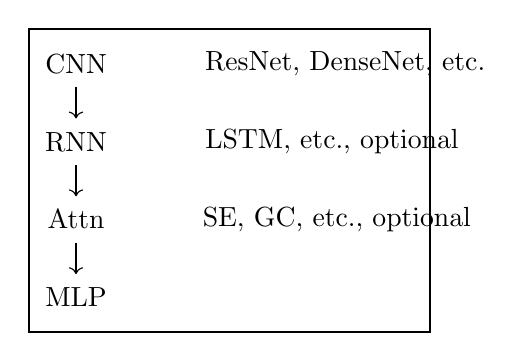
\begin{tikzpicture}[node distance = 1cm, auto]
\node[] (cnn) {CNN};
\node[right = 1cm of cnn.east] () {ResNet, DenseNet, etc.};
\node[below = 0.5cm of cnn.south] (rnn) {RNN};
\node[right = 1cm of rnn.east] () {LSTM, etc., optional};
\node[below = 0.5cm of rnn.south] (attn) {Attn};
\node[right = 1cm of attn.east] () {SE, GC, etc., optional};
\node[below = 0.5cm of attn.south] (mlp) {MLP};

\path[->] ([yshift = -0.05cm]cnn.south) edge ([yshift = 0.05cm]rnn.north);
\path[->] ([yshift = -0.05cm]rnn.south) edge ([yshift = 0.05cm]attn.north);
\path[->] ([yshift = -0.05cm]attn.south) edge ([yshift = 0.05cm]mlp.north);

\draw[thick] ([xshift=-0.6cm,yshift=0.2cm]cnn.north) rectangle ([xshift=4.5cm,yshift=-0.2cm]mlp.south);
\end{tikzpicture}

\end{center}

\vspace{-0.3cm}

For our challenge entries,

\vspace{-0.35cm}

\begin{itemize}
    \item explicitly model spectral characteristics via multi-branch CNNs each with different {\bf dilation} factor
    \vspace{-0.25cm}
    \item Attention module: SE (reduction=8)
\end{itemize}

Architecture of multi-branch CNNs:

\begin{center}

\scriptsize

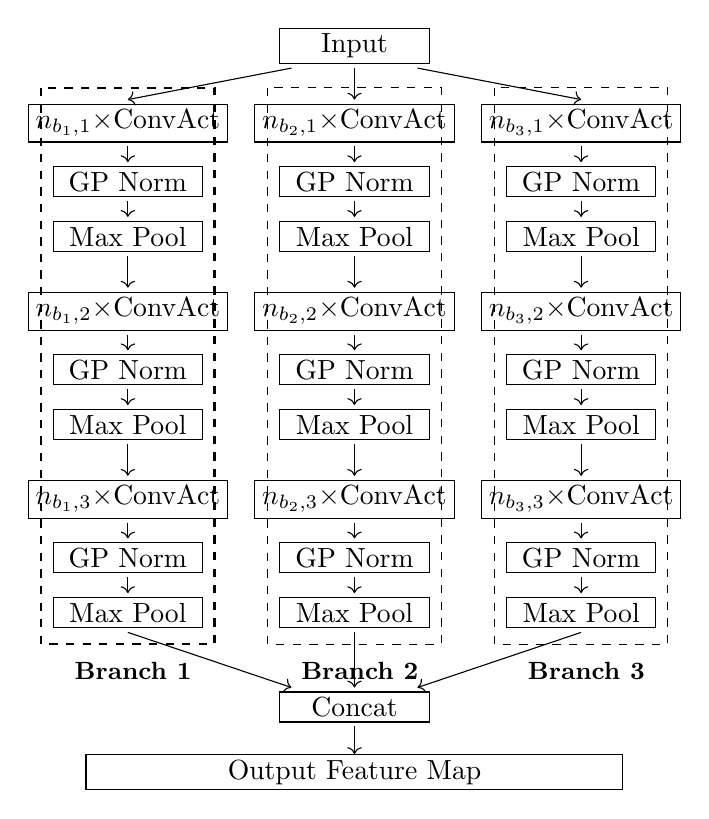
\begin{tikzpicture}[node distance = 1cm, auto]

% TODO: use for loops to simplify the code drawing the figure

\tikzstyle{block} = [rectangle, draw, text width = 5em, text centered, inner sep = 2pt, minimum height = 0.9em]

\tikzstyle{branchblock} = [rectangle, draw, text width = 6.8em, text centered, inner sep = 2pt, minimum height = 0.9em]

\tikzstyle{txt_block} = [rectangle, draw, text width = 19em, text centered, inner sep = 2pt, minimum height = 0.9em]

\node [block] (input) {Input};

% branch1
\node [branchblock, below left = 0.5cm and 0.65cm of input] (b1_ca1) {$n_{b_1,1}\times$ConvAct};
\node [block, below = 0.3cm of b1_ca1] (b1_bn1) {GP Norm};
\node [block, below = 0.3cm of b1_bn1] (b1_pool1) {Max Pool};
\node [branchblock, below = 0.5cm of b1_pool1] (b1_ca2) {$n_{b_1,2}\times$ConvAct};
\node [block, below = 0.3cm of b1_ca2] (b1_bn2) {GP Norm};
\node [block, below = 0.3cm of b1_bn2] (b1_pool2) {Max Pool};
\node [branchblock, below = 0.5cm of b1_pool2] (b1_ca3) {$n_{b_1,3}\times$ConvAct};
\node [block, below = 0.3cm of b1_ca3] (b1_bn3) {GP Norm};
\node [block, below = 0.3cm of b1_bn3] (b1_pool3) {Max Pool};

\draw[dashed,thick] ([xshift=-1.1cm,yshift=0.2cm]b1_ca1.north) rectangle ([xshift=1.1cm,yshift=-0.2cm]b1_pool3.south);

\node [below = 0.3cm of b1_pool3] (branch_txt_1) {\textbf{\fontsize{9.5pt}{9.5pt} \selectfont Branch 1}};

% branch2
\node [branchblock, below = 0.5cm of input] (b2_ca1) {$n_{b_2,1}\times$ConvAct};
\node [block, below = 0.3cm of b2_ca1] (b2_bn1) {GP Norm};
\node [block, below = 0.3cm of b2_bn1] (b2_pool1) {Max Pool};
\node [branchblock, below = 0.5cm of b2_pool1] (b2_ca2) {$n_{b_2,2}\times$ConvAct};
\node [block, below = 0.3cm of b2_ca2] (b2_bn2) {GP Norm};
\node [block, below = 0.3cm of b2_bn2] (b2_pool2) {Max Pool};
\node [branchblock, below = 0.5cm of b2_pool2] (b2_ca3) {$n_{b_2,3}\times$ConvAct};
\node [block, below = 0.3cm of b2_ca3] (b2_bn3) {GP Norm};
\node [block, below = 0.3cm of b2_bn3] (b2_pool3) {Max Pool};

\draw[dashed] ([xshift=-1.1cm,yshift=0.2cm]b2_ca1.north) rectangle ([xshift=1.1cm,yshift=-0.2cm]b2_pool3.south);

\node [below = 0.3cm of b2_pool3] (branch_txt_2) {\textbf{\fontsize{9.5pt}{9.5pt} \selectfont Branch 2}};

% branch3
\node [branchblock, below right = 0.5cm and 0.65cm of input] (b3_ca1) {$n_{b_3,1}\times$ConvAct};
\node [block, below = 0.3cm of b3_ca1] (b3_bn1) {GP Norm};
\node [block, below = 0.3cm of b3_bn1] (b3_pool1) {Max Pool};
\node [branchblock, below = 0.5cm of b3_pool1] (b3_ca2) {$n_{b_3,2}\times$ConvAct};
\node [block, below = 0.3cm of b3_ca2] (b3_bn2) {GP Norm};
\node [block, below = 0.3cm of b3_bn2] (b3_pool2) {Max Pool};
\node [branchblock, below = 0.5cm of b3_pool2] (b3_ca3) {$n_{b_3,3}\times$ConvAct};
\node [block, below = 0.3cm of b3_ca3] (b3_bn3) {GP Norm};
\node [block, below = 0.3cm of b3_bn3] (b3_pool3) {Max Pool};

\draw[dashed] ([xshift=-1.1cm,yshift=0.2cm]b3_ca1.north) rectangle ([xshift=1.1cm,yshift=-0.2cm]b3_pool3.south);

\node [below = 0.3cm of b3_pool3] (branch_txt_3) {\textbf{\fontsize{9.5pt}{9.5pt} \selectfont Branch 3}};

\node [block, below = 0.8cm of b2_pool3] (cat) {Concat};

\path[->] ([yshift = -0.05cm, xshift=-0.8cm]input.south) edge ([yshift = 0.05cm]b1_ca1.north);
\path[->] ([yshift = -0.05cm, xshift=0.8cm]input.south) edge ([yshift = 0.05cm]b3_ca1.north);
\path[->] ([yshift = -0.05cm]input.south) edge ([yshift = 0.05cm]b2_ca1.north);

\path[->] ([yshift = -0.05cm]b1_ca1.south) edge ([yshift = 0.05cm]b1_bn1.north);
\path[->] ([yshift = -0.05cm]b1_bn1.south) edge ([yshift = 0.05cm]b1_pool1.north);
\path[->] ([yshift = -0.05cm]b1_pool1.south) edge ([yshift = 0.05cm]b1_ca2.north);
\path[->] ([yshift = -0.05cm]b1_ca2.south) edge ([yshift = 0.05cm]b1_bn2.north);
\path[->] ([yshift = -0.05cm]b1_bn2.south) edge ([yshift = 0.05cm]b1_pool2.north);
\path[->] ([yshift = -0.05cm]b1_pool2.south) edge ([yshift = 0.05cm]b1_ca3.north);
\path[->] ([yshift = -0.05cm]b1_ca3.south) edge ([yshift = 0.05cm]b1_bn3.north);
\path[->] ([yshift = -0.05cm]b1_bn3.south) edge ([yshift = 0.05cm]b1_pool3.north);

\path[->] ([yshift = -0.05cm]b2_ca1.south) edge ([yshift = 0.05cm]b2_bn1.north);
\path[->] ([yshift = -0.05cm]b2_bn1.south) edge ([yshift = 0.05cm]b2_pool1.north);
\path[->] ([yshift = -0.05cm]b2_pool1.south) edge ([yshift = 0.05cm]b2_ca2.north);
\path[->] ([yshift = -0.05cm]b2_ca2.south) edge ([yshift = 0.05cm]b2_bn2.north);
\path[->] ([yshift = -0.05cm]b2_bn2.south) edge ([yshift = 0.05cm]b2_pool2.north);
\path[->] ([yshift = -0.05cm]b2_pool2.south) edge ([yshift = 0.05cm]b2_ca3.north);
\path[->] ([yshift = -0.05cm]b2_ca3.south) edge ([yshift = 0.05cm]b2_bn3.north);
\path[->] ([yshift = -0.05cm]b2_bn3.south) edge ([yshift = 0.05cm]b2_pool3.north);

\path[->] ([yshift = -0.05cm]b3_ca1.south) edge ([yshift = 0.05cm]b3_bn1.north);
\path[->] ([yshift = -0.05cm]b3_bn1.south) edge ([yshift = 0.05cm]b3_pool1.north);
\path[->] ([yshift = -0.05cm]b3_pool1.south) edge ([yshift = 0.05cm]b3_ca2.north);
\path[->] ([yshift = -0.05cm]b3_ca2.south) edge ([yshift = 0.05cm]b3_bn2.north);
\path[->] ([yshift = -0.05cm]b3_bn2.south) edge ([yshift = 0.05cm]b3_pool2.north);
\path[->] ([yshift = -0.05cm]b3_pool2.south) edge ([yshift = 0.05cm]b3_ca3.north);
\path[->] ([yshift = -0.05cm]b3_ca3.south) edge ([yshift = 0.05cm]b3_bn3.north);
\path[->] ([yshift = -0.05cm]b3_bn3.south) edge ([yshift = 0.05cm]b3_pool3.north);

\path[->] ([yshift = -0.05cm]b2_pool3.south) edge ([yshift = 0.05cm]cat.north);
\path[->] ([yshift = -0.05cm]b1_pool3.south) edge ([yshift = 0.05cm, xshift=-0.8cm]cat.north);
\path[->] ([yshift = -0.05cm]b3_pool3.south) edge ([yshift = 0.05cm, xshift=0.8cm]cat.north);

\node [txt_block, below = 0.4cm of cat] (out) {Output Feature Map};
\path[->] ([yshift = -0.05cm]cat.south) edge (out);

\end{tikzpicture}
\end{center}

\vspace{-0.7cm}

\begin{itemize}
    \item GP Norm: group (= \#leads) norm
    \vspace{-0.2cm}
    \item ConvAct: group conv. + ReLU
    \vspace{-0.2cm}
    \item Branch 1 no dilation, Branch 2 mild dilations, Branch 3 very large dilations
\end{itemize}

}

%----------------------------------------------------------------------------------------
% Detectors via Clinical Rules
%----------------------------------------------------------------------------------------

\headerbox{Detectors via Clinical Rules}{name=clinical, span=2, column=1, row=1, below=introduction}{
% finished
\begin{itemize}
\item ``Brady'': average heart rate $\leq$ 60 BPM or equivalently average RR-intervals $\geq$ 1s.
\vspace{-0.2cm}
\item ``LAD'' and ``RAD'': positivity checking of QRS complexes of leads I, aVF (the ``2-lead'' method); or of leads I, II, aVF (the ``3-lead'' method).
\vspace{-0.2cm}
\item ``LQRSV'': peak-to-peak amplitudes of more than 80\% of the QRS complexes are $\leq$ 0.5 mV in the limb leads (I, II, III, aVR, aVL, aVF), or $\leq$ 1 mV in the precordial leads (V1-V6). If R peak detection fails, amplitude check will be done within sliding windows of length 0.12s.
\vspace{-0.2cm}
\item ``PR'': raw ECGs are high-pass filtered with cutoff frequency 47 Hz, and spike (peak) detection with prominence threshold of 0.3 follows.
\end{itemize}
}


%----------------------------------------------------------------------------------------
%	Preprocessing, Augmentations
%----------------------------------------------------------------------------------------

\headerbox{Preprocessing and Augmentations For Training DNNs}{name=data, span=2, column=1, row=1, below=clinical}{
% finished
\begin{itemize}
    \item ECGs resampled to 500Hz, bandpassed (0.5-60Hz), and cropped or zero-padded to 10s.
    \vspace{-0.2cm}
    \item if ``LQRSV'' is not to be predicted, ECGs are normalized, otherwise not.
    % \vspace{-0.2cm}
    \item reduce overfit: random masking.
    \vspace{-0.2cm}
    \item reduce overconfidence: label smoothing.
\end{itemize}
}

%----------------------------------------------------------------------------------------
%	Training Setups
%----------------------------------------------------------------------------------------

\headerbox{Training Setups}{name=training,span=2,column=1,row=1, below=data}{
% finished
\begin{itemize}
    \item loss function: weighted binary cross entropy; class weights inverse proportional to \# records
    \vspace{-0.2cm}
    \item optimizer: AMSGrad variant of {\bf AdamW} with lr 0.001 (planed {\bf OneCycleLR} scheduler)
    \vspace{-0.2cm}
    \item train-val split: 80\% -- 20\%
    \vspace{-0.2cm}
    \item batch size 32 or 64; epoch number $\leq 30$ with early stopping
\end{itemize}
}


%----------------------------------------------------------------------------------------
%	Submission Results
%----------------------------------------------------------------------------------------

\headerbox{Submission Results}{name=submission, span=1, column=1, below=training}{
% finished
% \begin{center}
% \includegraphics[keepaspectratio,width=0.77\textwidth]{images/challenge_scores.pdf}
% \end{center}
{\large \color{red} figure here}

\vspace{-0.2cm}
2 configurations for challenge submissions:
\vspace{-0.2cm}
\begin{itemize}
    \item DNN (21-dim. out) + clinical-rule detector (5-dim. out) $\rightarrow$ 26-dim. out
    \vspace{-0.3cm}
    \item pure DNN (26-dim. out, with ``-ncr'' suffix)
\end{itemize}
}


%----------------------------------------------------------------------------------------
%	Offline Evaluation Results
%----------------------------------------------------------------------------------------

\headerbox{Offline Train-Eval Results}{name=offline, span=1, column=2, below=training}{
% finished
% \begin{center}
% \includegraphics[keepaspectratio,width=1\textwidth]{images/train.pdf}
% \end{center}
{\large \color{red} figure here}
\vspace{-0.3cm}
2 typical experiments on standard 12-lead set under the 2 configurations resp.
}


%----------------------------------------------------------------------------------------
%	Limitations, Discussions
%----------------------------------------------------------------------------------------

\headerbox{Limitations and Discussions}{name=discussion, column=0, below=nn, span=3}{
% finished
\begin{itemize} 
\item Reduced-lead ECGs, even 2-lead ECGs in the extreme case, provide sufficient information for making reliable auxiliary diagnoses.
\vspace{-0.2cm}
\item Multi-branch CNNs for feature extraction are far from optimal, whose structures and hyperparameters have to be optimized. Moreover, a thorough search for more effective architectures should be and is undertaken in our ECG deep learning framework.
\vspace{-0.2cm}
\item Hyperparameters of clinical rules based detectors are set empirically, which should be optimized via grid searches.
\vspace{-0.2cm}
\item Label heterogeneity (across datasets) and insufficiency (debate on labels) should also be noted.
\vspace{-0.2cm}
\item ``Lead-wise'' CNNs provides flexible light weight solutions to reduced-lead ECGs. Mechanism of parameters reuse is to be further established.
\end{itemize}
}


%----------------------------------------------------------------------------------------
%	REFERENCES
%----------------------------------------------------------------------------------------

%\headerbox{References}{name=references,column=2,below=application}{

%\smaller % Reduce the font size in this block
%\renewcommand{\section}[2]{\vskip 0.05em} % Get rid of the default "References" section title
%\nocite{*} % Insert publications even if they are not cited in the poster

%\bibliographystyle{unsrt}
%\bibliographystyle{IEEEtran}
%\bibliography{biblio} % Use biblio.bib as the bibliography file
%}


%----------------------------------------------------------------------------------------
%	ACKNOWLEDGEMENTS
%----------------------------------------------------------------------------------------

\headerbox{Acknowledgements}{name=acknowledgements, column=0, below=discussion, span=3}{
% finished
\smaller 
We would like to thank professor {\bf Deren Han} from the School of Mathematical Sciences, Beihang University and professor {\bf Wenjian Yu} from the Department of Computer Science and Technology, BNRist, Tsinghua University for generously providing GPU servers to help accomplish this work.

% \hfill \small \textit{Code, configs, etc. available at \href{https://github.com/DeepPSP/cinc2021}{https://github.com/DeepPSP/cinc2021}.}
}

%----------------------------------------------------------------------------------------
%	link to the github repository
%----------------------------------------------------------------------------------------

\headerbox{}{name=foottext, column=0, span=3, below=acknowledgements, textborder=none, headerborder=none,  boxheaderheight=0pt}{
% finished
\hfill \small \textit{Code, configs, etc. available at \href{https://github.com/DeepPSP/cinc2021}{https://github.com/DeepPSP/cinc2021}.}
}


\end{poster}

\end{document}
